\section{Bibliometric Analysis (RQ1)}
\label{sec:bibliometrics}

To address RQ1, this section quantifies publication volume, venue concentration, geographic collaboration, co-authorship topology, and decoupled orthogonal structural trends across the validated core corpus ($N=44$).

\subsection{Temporal Growth and Venue Disaggregation}
Scholarly output linking generative language models and digital forensics exhibits steep, non-linear growth between 2021 and late 2026. No peer-reviewed studies meeting eligibility criteria appeared in 2021 or 2022. Initial domain contributions emerged in 2023 with 3 publications (6.8\%: 2 journal articles and 1 workshop paper), anchored by conceptual analyses evaluating ChatGPT against investigative workflows~\cite{scanlon2023_digital, scanlon2023_chatgpt} and early LLM invocation-log forensics~\cite{chernyshev2023_towards}.

Volume increased modestly in 2024 to 4 papers (9.1\%: 2 journal articles and 2 conference papers), marking the transition toward empirical benchmarks on memory dumps, assisted report drafting, and multi-agent platform artifacts~\cite{oh2024_volgpt, michelet2024_chatgpt, walker2024_forensic}. A sharp inflection occurred during 2025 and 2026. Annual output expanded fourfold to 16 articles in 2025 (36.4\%: 8 journals and 8 proceedings) and reached 21 articles in 2026 year-to-date through November 10, 2026 (47.7\%: 10 journals and 11 proceedings). Together, 2025 and 2026 account for 84.1\% ($n=37$) of the corpus, split evenly across archival journals ($n=22$, 50.0\%) and peer-reviewed proceedings ($n=22$, 50.0\%). Fig.~\ref{fig:temporal_distribution} visualizes this annual trajectory disaggregated by publication type. Because 2026 indexing reflects a partial year, final 2026 volume will almost certainly exceed the observed peak.

\begin{figure}[!t]
\centering
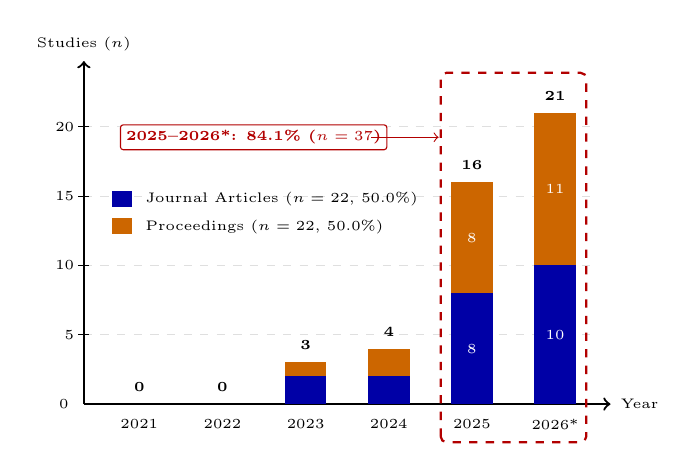
\begin{tikzpicture}[scale=0.88, font=\scriptsize]
  % Axes
  \draw[->, thick] (0,0) -- (7.6,0) node[right, font=\tiny] {Year};
  \draw[->, thick] (0,0) -- (0,4.95) node[above, font=\tiny] {Studies ($n$)};

  % Horizontal gridlines and y-ticks (scale: 1 unit = 5 articles -> y = n/5)
  \foreach \y/\lbl in {1/5, 2/10, 3/15, 4/20} {
    \draw[gray!25, dashed] (0,\y) -- (7.3,\y);
    \draw (-0.08,\y) -- (0.08,\y) node[left=2pt, font=\tiny] {\lbl};
  }
  \node[left=2pt, font=\tiny] at (0,0) {0};

  % Stacked bars: (x, journal_n, proc_n, total_lbl, year_lbl)
  % 2021: 0, 0
  \node[below=2pt, font=\tiny] at (0.8,0) {2021};
  \node[above=1pt, font=\tiny\bfseries] at (0.8,0) {0};

  % 2022: 0, 0
  \node[below=2pt, font=\tiny] at (2.0,0) {2022};
  \node[above=1pt, font=\tiny\bfseries] at (2.0,0) {0};

  % 2023: J=2 (0.4), P=1 (0.2), Total=3 (0.6)
  \fill[blue!65!black] (2.9,0) rectangle (3.5,0.4);
  \fill[orange!80!black] (2.9,0.4) rectangle (3.5,0.6);
  \node[below=2pt, font=\tiny] at (3.2,0) {2023};
  \node[above=1pt, font=\tiny\bfseries] at (3.2,0.6) {3};

  % 2024: J=2 (0.4), P=2 (0.4), Total=4 (0.8)
  \fill[blue!65!black] (4.1,0) rectangle (4.7,0.4);
  \fill[orange!80!black] (4.1,0.4) rectangle (4.7,0.8);
  \node[below=2pt, font=\tiny] at (4.4,0) {2024};
  \node[above=1pt, font=\tiny\bfseries] at (4.4,0.8) {4};

  % 2025: J=8 (1.6), P=8 (1.6), Total=16 (3.2)
  \fill[blue!65!black] (5.3,0) rectangle (5.9,1.6);
  \fill[orange!80!black] (5.3,1.6) rectangle (5.9,3.2);
  \node[white, font=\tiny] at (5.6,0.8) {8};
  \node[white, font=\tiny] at (5.6,2.4) {8};
  \node[below=2pt, font=\tiny] at (5.6,0) {2025};
  \node[above=1pt, font=\tiny\bfseries] at (5.6,3.2) {16};

  % 2026 YTD: J=10 (2.0), P=11 (2.2), Total=21 (4.2)
  \fill[blue!65!black] (6.5,0) rectangle (7.1,2.0);
  \fill[orange!80!black] (6.5,2.0) rectangle (7.1,4.2);
  \node[white, font=\tiny] at (6.8,1.0) {10};
  \node[white, font=\tiny] at (6.8,3.1) {11};
  \node[below=2pt, font=\tiny] at (6.8,0) {2026*};
  \node[above=1pt, font=\tiny\bfseries] at (6.8,4.2) {21};

  % Highlight bracket for 2025-2026 surge
  \draw[red!70!black, thick, dashed, rounded corners=2pt] (5.15,-0.55) rectangle (7.25,4.78);
  \node[fill=white, draw=red!70!black, rounded corners=1pt, font=\tiny\bfseries, text=red!70!black, inner sep=2pt] at (2.45,3.85) {2025--2026*: 84.1\% ($n=37$)};
  \draw[->, red!70!black, thin] (4.15,3.85) -- (5.12,3.85);

  % Legend
  \fill[blue!65!black] (0.4,2.85) rectangle (0.7,3.08);
  \node[right, font=\tiny] at (0.75,2.96) {Journal Articles ($n=22$, 50.0\%)};
  \fill[orange!80!black] (0.4,2.45) rectangle (0.7,2.68);
  \node[right, font=\tiny] at (0.75,2.56) {Proceedings ($n=22$, 50.0\%)};
\end{tikzpicture}
\caption{Annual publication trajectory of the validated corpus ($N=44$) disaggregated by publication venue type. *2026 reflects year-to-date Crossref indexing through November 10, 2026.}
\label{fig:temporal_distribution}
\end{figure}


\subsection{Dissemination Venues and Journal Concentration}
Publication outlets exhibit marked concentration within specialized digital forensics journals alongside selective penetration into flagship computer security conferences. Table~\ref{tab:venue_distribution} reports all recurring venues publishing two or more corpus studies.

\begin{table}[!t]
\caption{Publication Distribution Across Recurring Venues ($N=44$)}
\label{tab:venue_distribution}
\centering
\scriptsize
\begin{tabular}{p{4.8cm}cc}
\toprule
\textbf{Publication Venue} & \textbf{Articles ($n$)} & \textbf{Share (\%)} \\
\midrule
Forensic Science International: Digital Investigation (Elsevier) & 13 & 29.5\% \\
Journal of Forensic Sciences (Wiley) & 3 & 6.8\% \\
IEEE Int. Symp. on Digital Forensics and Security (ISDFS) & 3 & 6.8\% \\
Journal of Cybersecurity, Digital Forensics and Jurisprudence & 2 & 4.5\% \\
IEEE Annual COMPSAC Conference & 2 & 4.5\% \\
Single-Appearance Peer-Reviewed Journals \& Conferences* & 21 & 47.7\% \\
\midrule
\textbf{Total Validated Corpus} & \textbf{44} & \textbf{100.0\%}$^\dagger$ \\
\bottomrule
\multicolumn{3}{p{7.8cm}}{\tiny *Includes flagship venues with $n=1$ each: IEEE S\&P~\cite{xu2026_recovering}, NDSS~\cite{hammar2026_incident}, IEEE TIFS~\cite{zheng2025_avagent}, ACM SIGKDD~\cite{xu2025_enhancing}, ACM CIKM~\cite{xu2024_transforming}, IEEE/ACM ASE~\cite{tian2026_gala}, ACM DTRAP~\cite{michelet2025_finetuning}, and IEEE Access~\cite{kao2026_a}. $^\dagger$Individual rounded shares sum to 99.8\% due to single-decimal rounding.}
\end{tabular}
\end{table}

\textit{Forensic Science International: Digital Investigation} (FSIDI) dominates scholarly dissemination with 13 articles (29.5\%), reflecting strong domain gatekeeping by reviewers familiar with evidentiary reproducibility and custody standards. Specialized forums such as Wiley's \textit{Journal of Forensic Sciences} ($n=3$) and IEEE ISDFS ($n=3$) form a secondary tier. Crucially, the remaining 21 single-appearance outlets (47.7\%) are not peripheral; they include top-tier security and data-mining venues such as the IEEE Symposium on Security and Privacy (IEEE S\&P)~\cite{xu2026_recovering}, NDSS~\cite{hammar2026_incident}, IEEE Transactions on Information Forensics and Security (TIFS)~\cite{zheng2025_avagent}, ACM SIGKDD~\cite{xu2025_enhancing}, and IEEE/ACM ASE~\cite{tian2026_gala}, demonstrating mainstream security-community engagement with forensic LLM problems.

\subsection{Geographic, Institutional, and Citation Distribution}
Cross-validating all 44 DOIs against OpenAlex resolves Crossref's sparse affiliation reporting, raising structured institutional and geographic coverage from 61.4\% ($n=27$) in Crossref to 97.7\% ($n=43$ of 44 studies) in OpenAlex. Across these 43 affiliation-indexed publications, 18 countries are represented (Table~\ref{tab:geo_distribution}). Using full-counting attribution (crediting each participating country once per multi-country paper, totaling 56 country appearances), the United States leads with $n=17$ papers (39.5\% of affiliation-indexed works), followed by South Korea, Switzerland, and Ireland ($n=5$ each, 11.6\% each), Australia and Germany ($n=4$ each, 9.3\% each), and the United Kingdom ($n=3$, 7.0\%). Leading institutional contributors include University College Dublin ($n=5$), Louisiana State University ($n=4$), University of Lausanne ($n=4$), University of Baltimore ($n=3$), and Sungkyunkwan University ($n=3$). Multi-institutional co-authorship appears in 20 of 43 indexed papers (46.5\%), whereas cross-border international collaboration remains confined to 8 papers (18.6\%, e.g.,~\cite{michelet2025_finetuning, hammar2026_a, sava2026_triagecpg}), reflecting divergent statutory evidentiary frameworks across court jurisdictions.

\begin{table}[!t]
\caption{Geographic Distribution and Cross-Database Citation Impact ($n=43$ OpenAlex Affiliation-Indexed Papers; $N=44$ Corpus)}
\label{tab:geo_distribution}
\centering
\scriptsize
\begin{tabular}{p{3.9cm}cc}
\toprule
\textbf{Country / Bibliometric Indicator} & \textbf{Count ($n$)} & \textbf{Share (\%)} \\
\midrule
United States & 17 & 39.5\% \\
South Korea, Switzerland, Ireland & 5 each & 11.6\% each \\
Australia, Germany & 4 each & 9.3\% each \\
United Kingdom & 3 & 7.0\% \\
Turkey, Canada & 2 each & 4.7\% each \\
Other (CN, EG, ID, IN, JP, MA, NL, TW, IL) & 1 each & 2.3\% each \\
\midrule
Multi-Institutional Papers (of $n=43$) & 20 & 46.5\% \\
Cross-Border Collaborations (of $n=43$) & 8 & 18.6\% \\
\midrule
Crossref Citations ($N=44$, Sum / Mean / Med.) & 385 & 8.75 / 2.0 \\
OpenAlex Citations ($N=44$, Sum / Mean / Med.) & 903 & 20.52 / 4.0 \\
Uncited Papers (Crossref / OpenAlex) & 18 / 14 & 40.9\% / 31.8\% \\
\bottomrule
\multicolumn{3}{p{7.8cm}}{\tiny Note: Country counts employ full counting across 8 cross-border papers, yielding 56 country appearances across 43 affiliation-indexed studies (sum of shares exceeds 100\%). Citation triangulation compares Crossref (\texttt{is-referenced-by-count}) against OpenAlex (\texttt{cited\_by\_count}) on November 19, 2026.}
\end{tabular}
\end{table}

Cross-database citation triangulation confirms rapid scholarly uptake despite the recency of the corpus. Crossref records 385 cumulative citations (mean 8.75, median 2.0, maximum 74; 18 uncited [40.9\%]), whereas OpenAlex indexes 903 cumulative citations (mean 20.52, median 4.0, maximum 190; 14 uncited [31.8\%]). Across both indexes, impact concentrates heavily in early roadmaps and pioneer empirical benchmarks (reported as Crossref / OpenAlex citations): Scanlon et al.~\cite{scanlon2023_chatgpt} (74 / 190), Michelet and Breitinger~\cite{michelet2024_chatgpt} (41 / 92), Wickramasekara et al.~\cite{wickramasekara2025_exploring} (28 / 88), Jelodar et al.~\cite{jelodar2026_large} (31 / 81), Sharma et al.~\cite{sharma2025_forensicllm} (26 / 59), and Farber~\cite{farber2025_scpaiscp} (36 / 53).

\subsection{Co-Authorship Networks and Orthogonal Taxonomic Mapping}
Graph reconstruction of Crossref author metadata identifies 155 author appearances across 130 unique researchers (mean 3.52 authors per paper; 40 multi-authored [90.9\%] vs.\ 4 single-authored [9.1\%]). The collaboration network partitions into 30 connected components anchored by three productive clusters: a 13-author U.S.\ memory and agentic-forensics group centered on Baggili ($n=4$) and Gharaibeh ($n=3$)~\cite{sharma2025_forensicllm, gharaibeh2026_rusting, satter2026_with}; a 12-author European cluster linking University College Dublin, University of Lausanne, University of Augsburg, and the Netherlands Forensic Institute led by Scanlon ($n=6$) and Breitinger ($n=5$)~\cite{scanlon2023_digital, michelet2025_finetuning, studiawan2025_towards}; and a 9-author Baltimore/Towson group led by Xu ($n=3$)~\cite{xu2024_transforming, zhou2025_forensic, khatiwala2025_evaluating}.

To avoid conflating mutually exclusive themes with orthogonal architectural attributes, we code all 44 studies along two separated layers depicted in Fig.~\ref{fig:subdomain_matrix}. First, mutually exclusive thematic clustering partitions the corpus into six operational subdomains summing exactly to $N=44$: \textit{Evidence Triage, Reporting, and Datasets} leads with 40.9\% ($n=18$), covering report drafting, keyword expansion, graph extraction, multilingual chat triage, and dataset construction~\cite{michelet2024_chatgpt, chakir2025_forensicsdata, yoo2026_scpllmscp, johnson2026_aiassisted}; \textit{Incident Response, Logs, and Agentic SOC} accounts for 20.5\% ($n=9$), addressing multi-agent correlation, cloud log parsing, timeline evaluation, and response planning~\cite{liu2025_autobnb, hammar2026_incident, alharthi2025_llmpowered, studiawan2025_towards}; \textit{Malware Analysis and Reverse Engineering} represents 13.6\% ($n=6$), spanning behavioral system-call classification, Code Property Graphs, and APK analysis~\cite{clark2025_large, sava2026_triagecpg, zheng2025_avagent, ozyurt2026_llmorchestrated}; \textit{Forensics of LLM and Agentic Systems} captures 11.4\% ($n=5$), examining artifact recovery from AutoGen, MCP memory, mobile local LLMs, invocation logs, and AI investigative readiness~\cite{chernyshev2023_towards, walker2024_forensic, xu2026_recovering, satter2026_with, scanlon2026_investigation}; \textit{Volatile Memory Forensics (LLM-Assisted)} accounts for 6.8\% ($n=3$), focusing on ransomware RAM triage, Volatility migration, and privacy-preserving wallet memory analysis~\cite{oh2024_volgpt, gharaibeh2026_rusting, kao2026_a}; and \textit{Legal Admissibility, Explainability, and Covert Artifacts} accounts for 6.8\% ($n=3$), examining premise-acceptance bias, offline neuro-symbolic explainability, and LSB steganography~\cite{trivedi2026_when, tiwari2026_xforensicnet, sudheer2026_least}.

\begin{figure}[!t]
\centering
\resizebox{\columnwidth}{!}{%
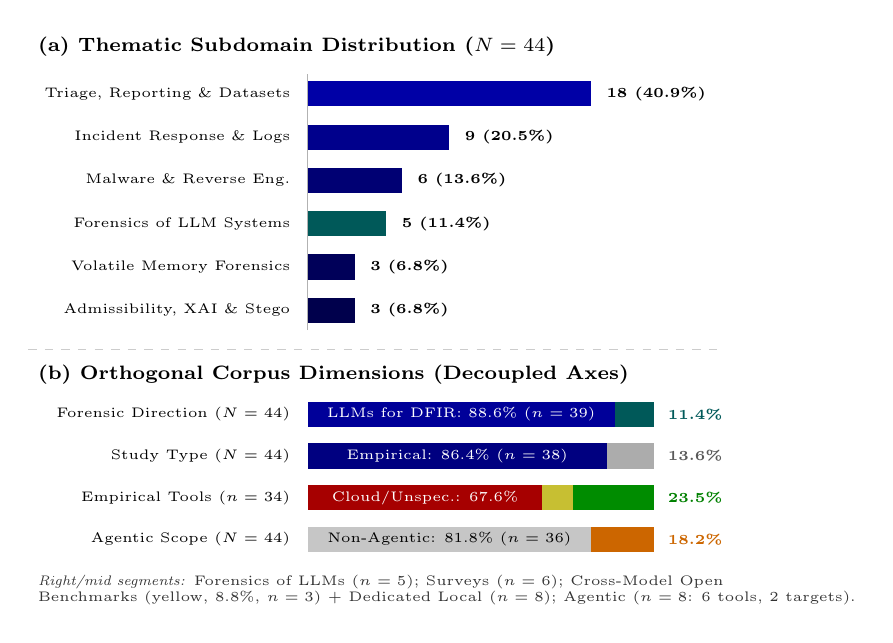
\begin{tikzpicture}[font=\scriptsize]
  % Panel A: Six Operational Subdomains (N=44)
  \node[anchor=west, font=\scriptsize\bfseries] at (0,5.25) {(a) Thematic Subdomain Distribution ($N=44$)};

  % Scale: 18 studies = 3.6 cm -> x = n * 0.20
  \foreach \y/\lbl/\n/\pct/\col in {
    4.65/{Triage, Reporting \& Datasets}/18/{40.9\%}/blue!65!black,
    4.10/{Incident Response \& Logs}/9/{20.5\%}/blue!55!black,
    3.55/{Malware \& Reverse Eng.}/6/{13.6\%}/blue!45!black,
    3.00/{Forensics of LLM Systems}/5/{11.4\%}/teal!70!black,
    2.45/{Volatile Memory Forensics}/3/{6.8\%}/blue!35!black,
    1.90/{Admissibility, XAI \& Stego}/3/{6.8\%}/blue!30!black%
  } {
    \node[anchor=east, font=\tiny] at (3.45,\y) {\lbl};
    \fill[\col] (3.55,\y-0.16) rectangle ({3.55+\n*0.20},\y+0.16);
    \node[anchor=west, font=\tiny\bfseries] at ({3.62+\n*0.20},\y) {\n\ (\pct)};
  }
  \draw[gray!60] (3.55,1.65) -- (3.55,4.90);

  % Divider
  \draw[gray!40, dashed] (0,1.40) -- (8.85,1.40);

  % Panel B: Orthogonal Structural Indicators (100% stacked horizontal bars, width = 4.4cm)
  \node[anchor=west, font=\scriptsize\bfseries] at (0,1.08) {(b) Orthogonal Corpus Dimensions (Decoupled Axes)};

  % Row 1: Forensic Direction (N=44): 39 (88.6%) vs 5 (11.4%)
  \node[anchor=east, font=\tiny] at (3.45,0.58) {Forensic Direction ($N=44$)};
  \fill[blue!60!black] (3.55,0.42) rectangle ({3.55+4.4*0.886},0.74);
  \fill[teal!70!black] ({3.55+4.4*0.886},0.42) rectangle ({3.55+4.4},0.74);
  \node[white, font=\tiny] at (5.50,0.58) {LLMs for DFIR: 88.6\% ($n=39$)};
  \node[anchor=west, font=\tiny\bfseries, text=teal!70!black] at (8.00,0.58) {11.4\%};

  % Row 2: Study Type (N=44): 38 (86.4%) vs 6 (13.6%)
  \node[anchor=east, font=\tiny] at (3.45,0.05) {Study Type ($N=44$)};
  \fill[blue!50!black] (3.55,-0.11) rectangle ({3.55+4.4*0.864},0.21);
  \fill[gray!65] ({3.55+4.4*0.864},-0.11) rectangle ({3.55+4.4},0.21);
  \node[white, font=\tiny] at (5.45,0.05) {Empirical: 86.4\% ($n=38$)};
  \node[anchor=west, font=\tiny\bfseries, text=gray!70!black] at (8.00,0.05) {13.6\%};

  % Row 3: Empirical DFIR Tools (n=34): Cloud/Unspec 23 (67.6%) + Cross-Model Open 3 (8.8%) + Dedicated Local 8 (23.5%)
  \node[anchor=east, font=\tiny] at (3.45,-0.48) {Empirical Tools ($n=34$)};
  \fill[red!65!black] (3.55,-0.64) rectangle ({3.55+4.4*0.676},-0.32);
  \fill[yellow!75!black] ({3.55+4.4*0.676},-0.64) rectangle ({3.55+4.4*0.765},-0.32);
  \fill[green!55!black] ({3.55+4.4*0.765},-0.64) rectangle ({3.55+4.4},-0.32);
  \node[white, font=\tiny] at (5.04,-0.48) {Cloud/Unspec.: 67.6\%};
  \node[anchor=west, font=\tiny\bfseries, text=green!50!black] at (8.00,-0.48) {23.5\%};

  % Row 4: Orchestration (N=44): Non-Agentic 36 (81.8%) vs Agentic 8 (18.2%)
  \node[anchor=east, font=\tiny] at (3.45,-1.01) {Agentic Scope ($N=44$)};
  \fill[gray!45] (3.55,-1.17) rectangle ({3.55+4.4*0.818},-0.85);
  \fill[orange!80!black] ({3.55+4.4*0.818},-1.17) rectangle ({3.55+4.4},-0.85);
  \node[black, font=\tiny] at (5.35,-1.01) {Non-Agentic: 81.8\% ($n=36$)};
  \node[anchor=west, font=\tiny\bfseries, text=orange!80!black] at (8.00,-1.01) {18.2\%};

  % Compact two-line legend for right-hand & middle segments
  \node[anchor=west, font=\tiny, text=black!80, align=left] at (0,-1.65) {\textit{Right/mid segments:} Forensics of LLMs ($n=5$); Surveys ($n=6$); Cross-Model Open\\Benchmarks (yellow, 8.8\%, $n=3$) + Dedicated Local ($n=8$); Agentic ($n=8$: 6 tools, 2 targets).};
\end{tikzpicture}%
}
\caption{Thematic subdomain ranking and decoupled orthogonal structural indicators across the validated corpus ($N=44$), verified via Crossref and OpenAlex (40/44 abstracts/full texts). Deployment locality is evaluated strictly over empirical LLM-for-DFIR tool studies ($n=34$).}
\label{fig:subdomain_matrix}
\end{figure}


Second, decoupled orthogonal coding separates four independent structural dimensions across the corpus. Along the \textit{Forensic Direction} axis, 88.6\% ($n=39$) apply LLMs as DFIR instruments whereas 11.4\% ($n=5$) examine LLM platforms as forensic subjects. Along the \textit{Study Type} axis, 86.4\% ($n=38$) present empirical implementations, benchmarks, datasets, or artifact studies, whereas 13.6\% ($n=6$) are conceptual roadmaps, surveys, or readiness reviews~\cite{scanlon2023_digital, scanlon2023_chatgpt, wickramasekara2025_exploring, chernyshev2026_large, jelodar2026_large, scanlon2026_investigation}. Measuring \textit{Deployment Locality} strictly over the $n=34$ empirical LLM-for-DFIR tool studies (excluding six surveys and four empirical LLM-as-subject studies to avoid denominator inflation, verified across 40/44 abstracts and full texts) reveals three distinct tiers: only 23.5\% ($n=8$) design, fine-tune, or deploy dedicated local, offline, or lightweight open-weights models~\cite{sharma2025_forensicllm, michelet2024_chatgpt, michelet2025_finetuning, tiwari2026_xforensicnet, kao2026_a, hammar2026_incident, hammar2026_a, clark2025_large}, another 8.8\% ($n=3$) include open-weights baselines within multi-model comparative benchmarks~\cite{chakir2025_forensicsdata, studiawan2025_towards, sava2026_triagecpg}, and the remaining 67.6\% ($n=23$) rely on commercial cloud APIs or omit explicit local air-gapped deployment guarantees. Independently, along the \textit{Agentic Orchestration} axis, 18.2\% ($n=8$) of the corpus engages agentic architectures: 13.6\% ($n=6$) implement multi-agent DFIR or malware pipelines~\cite{liu2025_autobnb, ozyurt2026_llmorchestrated, zgzler2026_eventdriven, tian2026_gala, zheng2025_avagent, tiwari2026_xforensicnet}, and 4.5\% ($n=2$) perform forensic artifact recovery on agentic frameworks~\cite{walker2024_forensic, satter2026_with}.

To verify structural robustness against inclusion-boundary choices, we performed a formal sensitivity analysis excluding all five borderline records simultaneously: the two domain-adjacent studies~\cite{farber2025_scpaiscp, tian2026_gala} and the three short archival papers under four pages~\cite{xu2025_enhancing, sudheer2026_least, hammar2026_a} (including the companion NOMS demo to~\cite{hammar2026_incident}). Across the resulting strict subset ($N_{\text{sens}}=39$, with $n_{\text{emp}}=29$ empirical LLM-for-DFIR tools), the 2025--2026 YTD surge shifts marginally from 84.1\% to 82.1\% ($32/39$), dedicated local/offline tool adoption shifts from 23.5\% to 24.1\% ($7/29$), and cloud/unspecified reliance shifts from 67.6\% to 65.5\% ($19/29$). Every central bibliometric and architectural conclusion remains invariant within 2.1 percentage points. The complete study-by-study coding matrix is tabulated in the Appendix (Table~\ref{tab:master_corpus}).

\subsection{Evaluation Rigor and Benchmark Ground-Truth Audit}
Validating forensic AI claims requires realistic, noise-polluted ground-truth corpora reflecting operational casework rather than clean conversational prompts. Auditing dataset provenance across the open-access empirical subset (Table~\ref{tab:qa_audit}) alongside verifiable dataset disclosures in the broader corpus reveals three distinct empirical tiers. At the lowest external-validity tier, numerous evaluations depend on synthetic logs, fictive mini-cases, or isolated lab scenarios lacking concurrent background noise and corrupted filesystem metadata; within our six audited open-access empirical PDFs, Michelet and Breitinger~\cite{michelet2024_chatgpt} rely on a fictive DFRWS-reviewed case and Hammar et al.~\cite{hammar2026_incident} combine testbed telemetry with LLM-expanded synthetic incident data. At the intermediate tier, closed institutional or law-enforcement casework (e.g.,~\cite{kim2025_digital, ko2026_humansupervised}) offers operational realism but remains sealed under statutory privacy restrictions, precluding independent scientific replication. At the highest reproducibility tier, standardized public corpora remain comparatively scarce: among our six audited full texts, Chakir and Lahsen-Cherif~\cite{chakir2025_forensicsdata} contribute over 5,000 Question-Context-Answer triplets sourced from real malware reports, Khatiwala et al.~\cite{khatiwala2025_evaluating} evaluate a public 13~GB Capture-the-Flag disk image (61 applications, 2,864 databases, 5,870 tables), and Studiawan et al.~\cite{studiawan2025_towards} introduce a standardized timeline evaluation dataset modeled on the NIST Computer Forensics Tool Testing (CFTT) program~\cite{nist_cftt}. Conversely, direct benchmarking against established NIST Computer Forensic Reference Data Sets (CFReDS)~\cite{nist_cfreds} remains conspicuously rare across the corpus. High precision on clean synthetic excerpts therefore provides no guarantee against retrieval collapse on unfiltered, multi-terabyte enterprise images.
